\documentclass{article}
\usepackage[utf8]{inputenc}
\usepackage[spanish]{babel}
\usepackage{amsmath}
\usepackage{amssymb}
\usepackage{graphicx}
\usepackage{geometry} % Para ajustar los márgenes
\usepackage{float} % Para la opción de flotante H
\usepackage{listings} % Para resaltar el código
\usepackage{xcolor} % Para colores en el código
\usepackage{enumitem} % Para mejorar las listas

% Configuración de los márgenes
\geometry{a4paper, left=2.5cm, right=2.5cm, top=2.5cm, bottom=2.5cm}

% Configuración del paquete listings
\lstset{
    frame=single, % Añade un cuadro alrededor del código
    basicstyle=\ttfamily\small, % Estilo de la fuente
    backgroundcolor=\color{gray!10}, % Color de fondo
    keywordstyle=\color{blue}, % Color de las palabras clave
    commentstyle=\color{green!50!black}, % Color de los comentarios
    stringstyle=\color{red}, % Color de las cadenas
    numbers=left, % Números de línea a la izquierda
    numberstyle=\tiny\color{gray}, % Estilo de los números de línea
    breaklines=true, % Romper líneas largas
    showstringspaces=false, % No mostrar espacios en cadenas
    tabsize=4 % Tamaño de la tabulación
}

\title{Proyecto de Optimización Lineal para la Planificación de Plantas de Generación Eléctrica}
\author{Noel Pérez Calvo (C311)\\ Jabel Resendiz Aguirre (C312)}
\date{}
\begin{document}

\maketitle

\section*{Definición del Problema}
En este proyecto se busca optimizar la planificación de la construcción y operación de plantas de generación eléctrica, minimizando los costos totales de construcción y operación, mientras se cumplen ciertas restricciones, como la demanda energética y las emisiones de CO$_2$.

\subsection*{Datos del Problema}
El problema incluye tres tipos de plantas:
\begin{itemize}[noitemsep]
    \item Térmica (T)
    \item Hidroeléctrica (H)
    \item Renovable (R)
\end{itemize}
Cada tipo de planta tiene costos asociados de construcción y operación, así como emisiones de CO$_2$. Además, hay límites en la cantidad mínima y máxima de generación de cada planta y restricciones en el número de plantas a construir.

\begin{itemize}[noitemsep]
    \item Costos de construcción y generación:
    \begin{align*}
        &\text{Térmica: } 1,000,000 \text{ USD, 50 USD/MW} \\
        &\text{Hidroeléctrica: } 2,000,000 \text{ USD, 30 USD/MW} \\
        &\text{Renovable: } 800,000 \text{ USD, 20 USD/MW}
    \end{align*}
    \item Restricciones:
    \begin{itemize}[noitemsep]
        \item Demanda total: 1000 MW.
        \item Límite de emisiones de CO$_2$: 500 toneladas.
    \end{itemize}
\end{itemize}



\subsection*{Variables}
Se definen las siguientes variables:
\begin{itemize}[noitemsep]
    \item $x_T, x_H, x_R \in \mathbb{Z}^+$: Número de plantas a construir de cada tipo.
    \item $g_{Ti}, g_{Hj}, g_{Rk} \geq 0$: Generación de cada planta térmica, hidroeléctrica y renovable.
\end{itemize}

\subsection*{Función Objetivo}
La función objetivo busca minimizar el costo total de construcción y operación de las plantas de generación:
\[
\min Z = \sum_{i=1}^{x_T} (1,000,000) + \sum_{j=1}^{x_H} (2,000,000) + \sum_{k=1}^{x_R} (800,000) + \sum_{i=1}^{x_T} (50 g_{Ti}) + \sum_{j=1}^{x_H} (30 g_{Hj}) + \sum_{k=1}^{x_R} (20 g_{Rk})
\]

\subsection*{Restricciones}
\begin{itemize}[noitemsep]
    \item Demanda energética: 
    \[
    \sum_{i=1}^{x_T} g_{Ti} + \sum_{j=1}^{x_H} g_{Hj} + \sum_{k=1}^{x_R} g_{Rk} \geq 1000
    \]
    \item Restricciones de generación por planta:
    \[
    50 \leq g_{Ti} \leq 200, \quad 100 \leq g_{Hj} \leq 300, \quad 20 \leq g_{Rk} \leq 150
    \]
    \item Límite de emisiones de CO$_2$:
    \[
    \sum_{i=1}^{x_T} 0.8 g_{Ti} \leq 500
    \]
\end{itemize}

\section*{Estrategia de Resolución}
El problema se resolverá en dos fases:

\begin{enumerate}[noitemsep]
    \item \textbf{Fase 1:} Resolver el problema relajado utilizando el método Simplex.
    \item \textbf{Fase 2:} Resolver el problema utilizando Ramificación y Acotación (Branch \& Bound).
\end{enumerate}

\section*{Fase 1: Resolución con el Método Simplex Relajado}
En esta fase, se resuelve el problema sin considerar la restricción de enteros, utilizando el método Simplex. El problema se modela como un problema de programación lineal con variables continuas.
\\
\begin{lstlisting}[language=Python, literate={á}{{\'a}}1 {é}{{\'e}}1 {í}{{\'i}}1 {ó}{{\'o}}1 {ú}{{\'u}}1 {ñ}{{\~n}}1]
import pulp
import matplotlib.pyplot as plt
import numpy as np

# Definir el problema
problem = pulp.LpProblem("LP_PowerPlant_Optimization", pulp.LpMinimize)

# Variables continuas para la cantidad de plantas
x_T = pulp.LpVariable("x_T", lowBound=0, upBound=10, cat='Continuous')
x_H = pulp.LpVariable("x_H", lowBound=0, upBound=10, cat='Continuous')
x_R = pulp.LpVariable("x_R", lowBound=0, upBound=10, cat='Continuous')

# Variables continuas para la generacion por planta
G_T = pulp.LpVariable("G_T", lowBound=0)
G_H = pulp.LpVariable("G_H", lowBound=0)
G_R = pulp.LpVariable("G_R", lowBound=0)

# Restringir G_T, G_H, G_R segun las plantas
problem += G_T >= 50 * x_T
problem += G_T <= 200 * x_T
problem += G_H >= 100 * x_H
problem += G_H <= 300 * x_H
problem += G_R >= 20 * x_R
problem += G_R <= 150 * x_R

# Función objetivo: Minimizar costos totales
problem += (
    x_T * 1_000_000 + x_H * 2_000_000 + x_R * 800_000 +
    50 * G_T + 30 * G_H + 20 * G_R
), "Total_Cost"

# Restricción de demanda
problem += (G_T + G_H + G_R >= 1000), "Demand"

# Restricción de emisiones de CO2
problem += (0.8 * G_T <= 500), "CO2_Limit"

# Resolver el problema con Simplex
problem.solve()

# Imprimir resultados
print("Estado de la solución:", pulp.LpStatus[problem.status])
print("Costo total:", pulp.value(problem.objective))
print("Plantas térmicas:", pulp.value(x_T))
print("Plantas hidroeléctricas:", pulp.value(x_H))
print("Plantas renovables:", pulp.value(x_R))
print("Generación térmica:", pulp.value(G_T))
print("Generación hidroeléctrica:", pulp.value(G_H))
print("Generación renovable:", pulp.value(G_R))

# Visualización de la generación 
labels = ["Térmica", "Hidroeléctrica", "Renovable"]
generacion = [pulp.value(x_T), pulp.value(x_H), pulp.value(x_R)]

plt.figure(figsize=(8, 6))
plt.bar(labels, generacion, color=['red', 'blue', 'green'])
plt.xlabel("Tipo de Planta")
plt.ylabel("Generación (MW)")
plt.title("Distribución de la Generación de Energía")
plt.show()
\end{lstlisting}

\subsection*{Resultados}
\begin{itemize}[noitemsep]
    \item Estado de la solución: Óptima.
    \item Costo total: 5,163,750 USD.
    \item Plantas térmicas: 3.125.
    \item Plantas hidroeléctricas: 0.0.
    \item Plantas renovables: 2.5.
\end{itemize}

\begin{figure}[H]
    \centering
    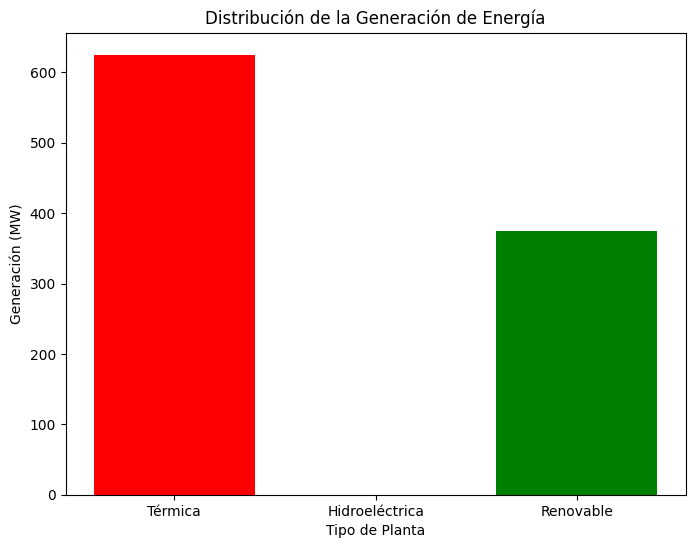
\includegraphics[width=0.8\textwidth]{simplex.png}
    \caption{Distribución de la generación de energía por tipo de planta}
\end{figure}


\section*{Fase 2: Resolución con Ramificación y Acotación}
En esta fase, se utiliza el método de Ramificación y Acotación para manejar las restricciones de enteros en las variables. A continuación, se muestra la implementación en Python del método:

\begin{lstlisting}[language=Python, literate={á}{{\'a}}1 {é}{{\'e}}1 {í}{{\'i}}1 {ó}{{\'o}}1 {ú}{{\'u}}1 {ñ}{{\~n}}1]
    import pulp
    import time
    import pandas as pd
    import matplotlib.pyplot as plt
    
    def branch_and_bound(problem, vars_ent, max_iters=100):
        """ Implementación del método Branch and Bound """
        iteraciones = 0
        cola = [(problem, [])]  # Inicializar la cola con el problema original
    
        mejor_sol = None
        mejor_costo = float("inf")
    
        while cola and iteraciones < max_iters:
            iteraciones += 1
            nodo, ramas = cola.pop(0)
    
            # Resolver la relajación LP del nodo actual
            nodo.solve()
    
            if nodo.status != pulp.LpStatusOptimal:
                continue  # No hay solución óptima para este nodo
    
            # Obtener solución óptima relajada
            costo_actual = pulp.value(nodo.objective)
            valores_vars = {var.name: pulp.value(var) for var in vars_ent}
    
            # Si la solución es peor que la mejor encontrada, descartar
            if costo_actual >= mejor_costo:
                continue
    
            # Verificar si todas las variables enteras están en valores enteros
            if all(abs(val - int(val)) < 1e-6 for val in valores_vars.values()):
                mejor_sol = valores_vars
                mejor_costo = costo_actual
                continue  # No hay necesidad de seguir explorando
    
            # Seleccionar una variable no entera para bifurcar
            var_frac = next(var for var in vars_ent if abs(valores_vars[var.name] - int(valores_vars[var.name])) > 1e-6)
    
            # Crear dos nuevos subproblemas con restricciones adicionales
            nuevo_nodo1 = nodo.deepcopy()
            nuevo_nodo1 += var_frac <= int(valores_vars[var_frac.name])
    
            nuevo_nodo2 = nodo.deepcopy()
            nuevo_nodo2 += var_frac >= int(valores_vars[var_frac.name]) + 1
    
            cola.append((nuevo_nodo1, ramas + [f"{var_frac.name} <= {int(valores_vars[var_frac.name])}"]))
            cola.append((nuevo_nodo2, ramas + [f"{var_frac.name} >= {int(valores_vars[var_frac.name]) + 1}"]))
    
        return mejor_sol, mejor_costo, iteraciones
    
    
    # ** Definir el problema inicial **
    def crear_problema():
        problem = pulp.LpProblem("MILP_PowerPlant_Optimization", pulp.LpMinimize)
    
        x_T = pulp.LpVariable("x_T", lowBound=0, upBound=10, cat='Continuous')
        x_H = pulp.LpVariable("x_H", lowBound=0, upBound=10, cat='Continuous')
        x_R = pulp.LpVariable("x_R", lowBound=0, upBound=10, cat='Continuous')
    
        G_T = pulp.LpVariable("G_T", lowBound=0)
        G_H = pulp.LpVariable("G_H", lowBound=0)
        G_R = pulp.LpVariable("G_R", lowBound=0)
    
        problem += G_T >= 50 * x_T
        problem += G_T <= 200 * x_T
        problem += G_H >= 100 * x_H
        problem += G_H <= 300 * x_H
        problem += G_R >= 20 * x_R
        problem += G_R <= 150 * x_R
    
        problem += (x_T * 1_000_000 + x_H * 2_000_000 + x_R * 800_000 +
                    50 * G_T + 30 * G_H + 20 * G_R), "Total_Cost"
    
        problem += (G_T + G_H + G_R >= 1000), "Demand"
        problem += (0.8 * G_T <= 500), "CO2_Limit"
    
        return problem, [x_T, x_H, x_R]
    
    
    if __name__ == "__main__":
        problema, vars_ent = crear_problema()
        
        start_time = time.time()
        solucion, costo, iteraciones = branch_and_bound(problema, vars_ent)
        end_time = time.time()
    
        tiempo_total = end_time - start_time
    
        print("\n **Resultados Branch and Bound**")
        print(f" Costo Optimo: {costo}")
        print(f" Iteraciones: {iteraciones}")
        print(f" Tiempo de ejecución: {tiempo_total:.4f} segundos")
        print(f" Solución óptima encontrada: {solucion}")
    
        # ** Visualización de generación de energía **
        if solucion:
            etiquetas = ["Térmica", "Hidroeléctrica", "Renovable"]
            valores = [solucion["x_T"], solucion["x_H"], solucion["x_R"]]
    
            plt.figure(figsize=(8, 6))
            plt.bar(etiquetas, valores, color=['red', 'blue', 'green'])
            plt.xlabel("Tipo de Planta")
            plt.ylabel("Cantidad de Plantas")
            plt.title("Distribución de la Generación de Energía - Branch and Bound")
            plt.show()
    
\end{lstlisting}
\subsection*{Resultados}
\begin{itemize}
    \item Estado de la solución: Óptima.
    \item Costo total: 5232000.0 USD.
    \item Plantas térmicas: 2.0.
    \item Plantas hidroeléctricas: 0.0.
    \item Plantas renovables: 4.0.
\end{itemize} 

\begin{figure}[H]
    \centering
    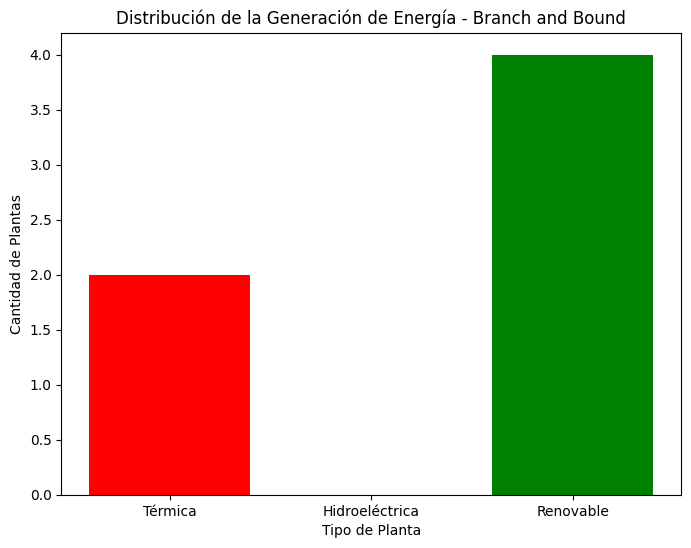
\includegraphics[width=0.8\textwidth]{BranchAndBound.png}
\caption{Distribución de la generación de energía por tipo de planta}
\end{figure}

\end{document}